\chapter{A/B 测试实验}
\label{chap:ab-test}

本章在真实 WebRTC 端到端链路上对离线强化学习策略与浏览器默认 GCC 算法进行 A/B 对比实验，验证第五章所得 IQL 策略在真实网络中的有效性，并讨论其适用边界。

\section{实验设计与数据采集}

本研究将浏览器端默认启用的 Google Congestion Control（GCC）作为对照组，将基于 IQL 训练得到的 Actor 策略作为实验组。两者的核心差异在于：GCC 依据接收端时延梯度与丢包反馈进行启发式调整，而 IQL 策略在每个控制周期根据状态窗口直接输出带宽上限，并通过 \texttt{RTCRtpSender.setParameters()} 施加为 \texttt{maxBitrate}，由此构成“策略输出—发送端限速—网络反馈—下一步决策”的闭环。为避免推理链路与媒体流共享网络信道导致控制滞后，A/B 测试统一采用浏览器端 ONNX 本地推理。

为降低在线对比的试错成本，实验组的模型以离线验证集 NLL 最优为准则进行选择。考虑到高斯策略的训练目标与验证指标均以对数似然为核心，NLL 更能反映策略对离线数据分布的拟合质量；故选取 NLL 最低对应的 \texttt{checkpoint\_50000} 导出 \texttt{actor.onnx} 作为部署模型，以获得更稳定、可解释的策略行为。

A/B 测试完全复用第四章 4.1.2 节定义的九类网络环境及其 \texttt{pfctl + dummynet} 参数配置。各静态场景的关键参数总览如图~\ref{fig:network-condition-parameter} 所示；其中 \texttt{fluctuating} 为动态时变场景，其参数沿时间轴的配置如图~\ref{fig:fluctuating-parameters} 所示，用于模拟带宽骤降与短时恢复等真实弱网波动。

\begin{figure}[htbp]
    \centering
    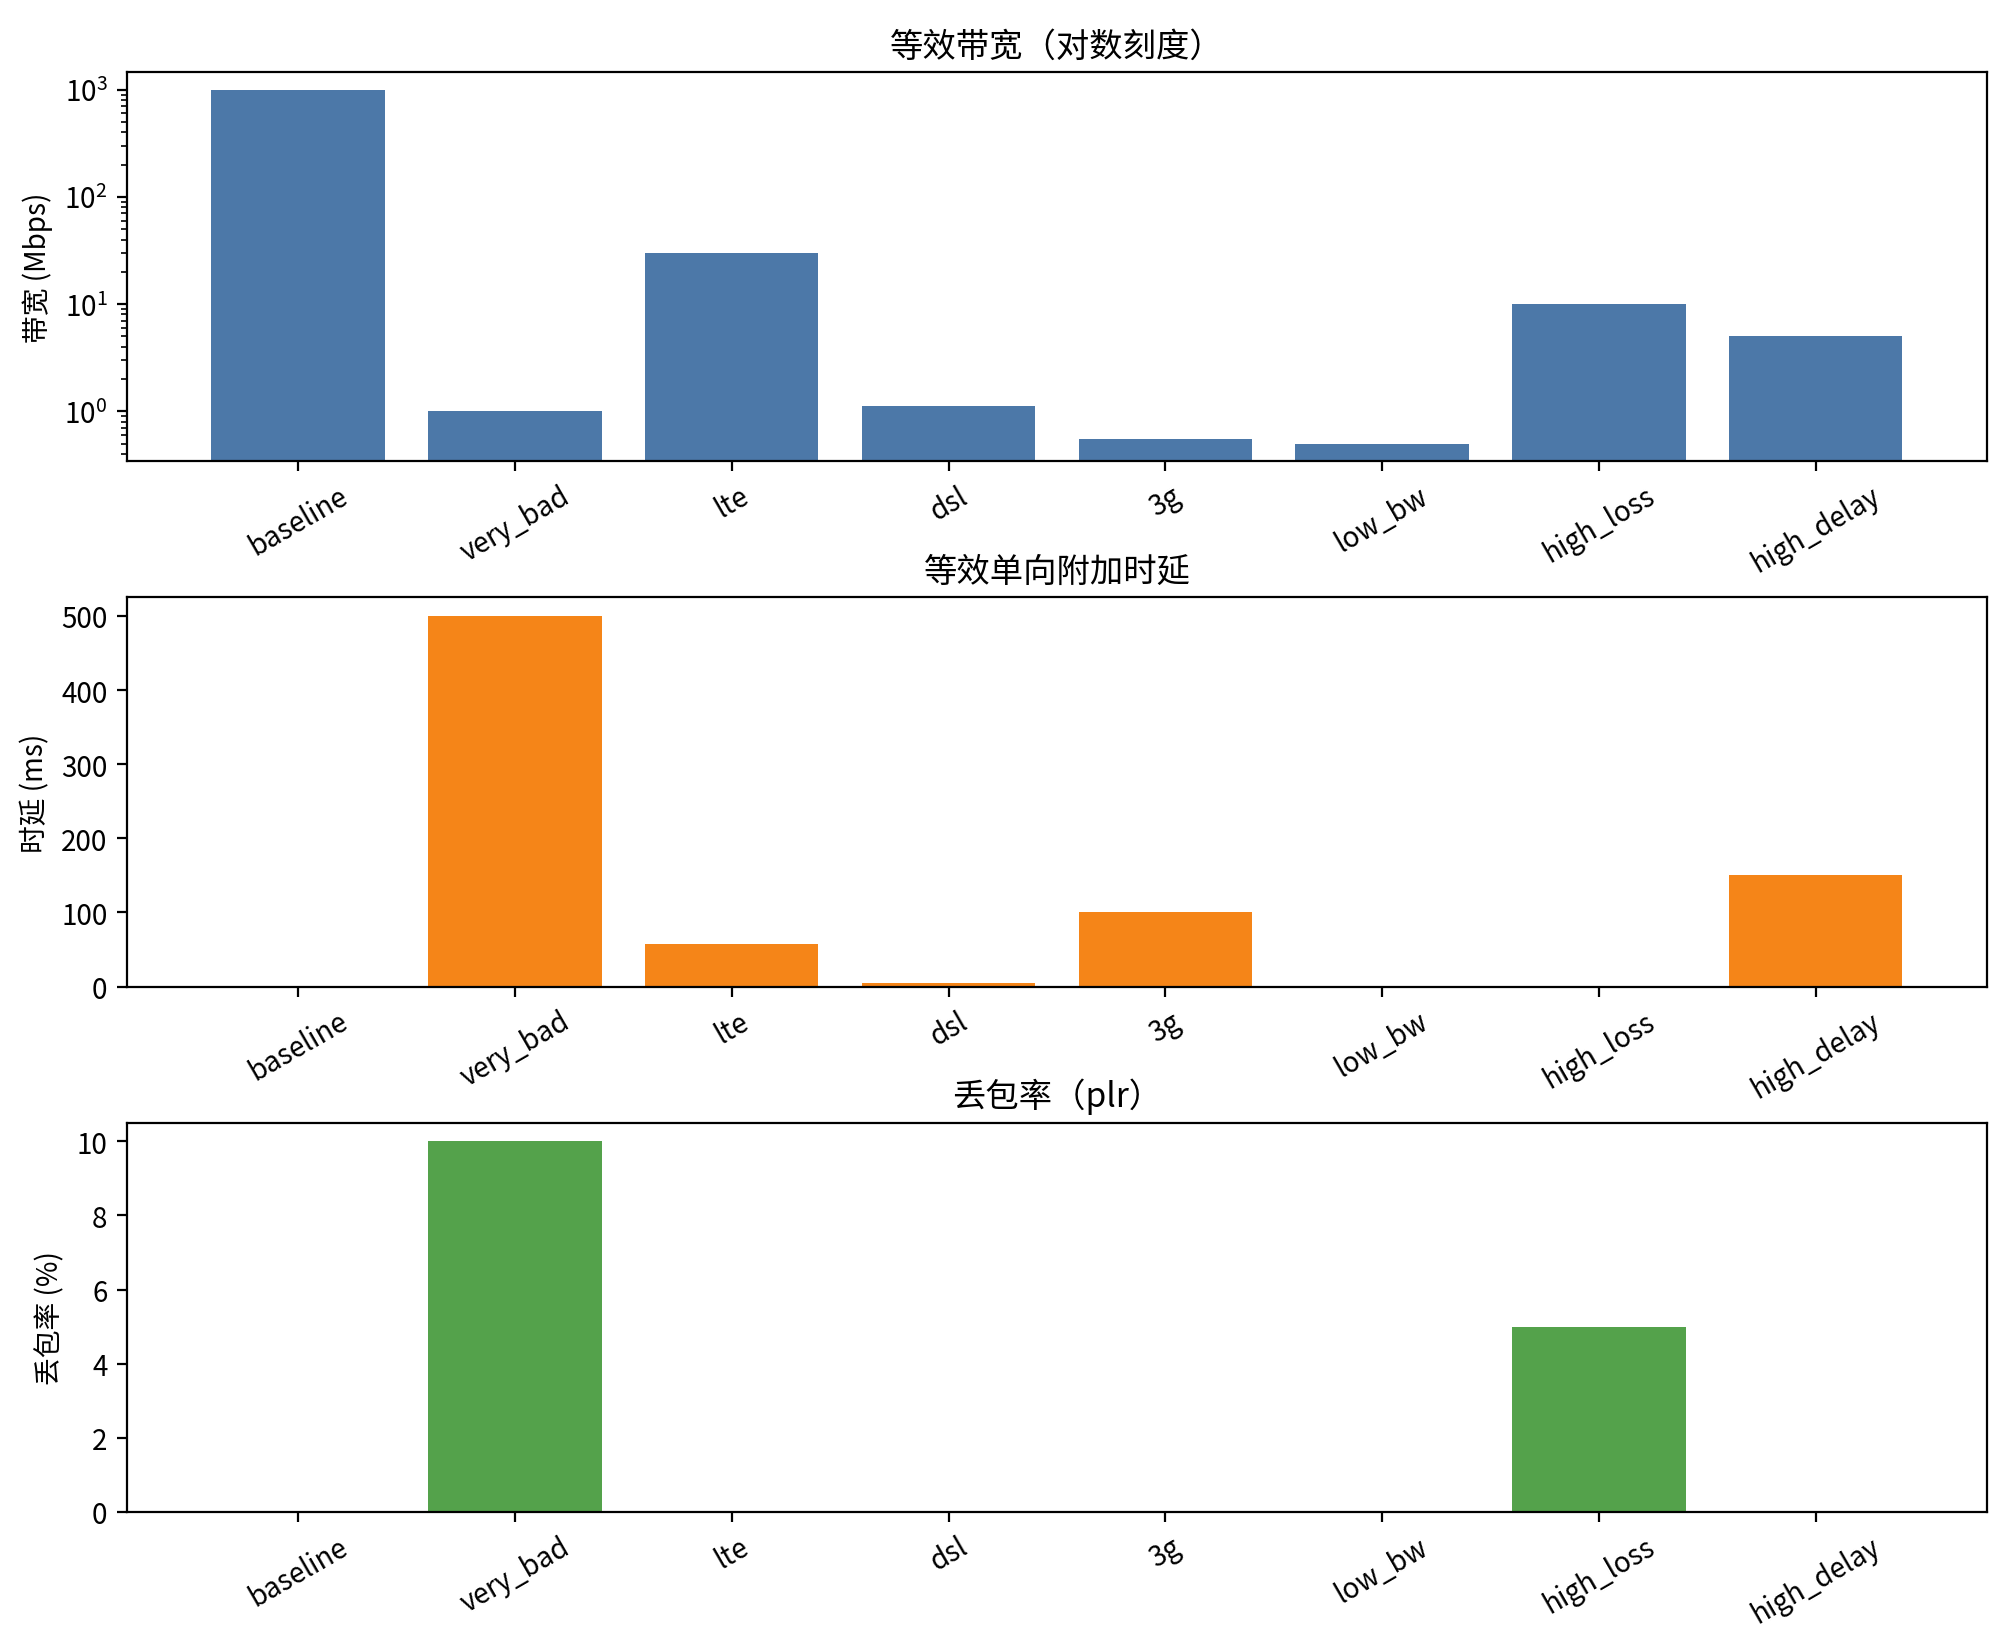
\includegraphics[width=0.95\textwidth]{figures/chapter6/network_condition_parameter.png}
    \caption{网络场景参数总览（静态场景）}
    \label{fig:network-condition-parameter}
\end{figure}

\begin{figure}[htbp]
    \centering
    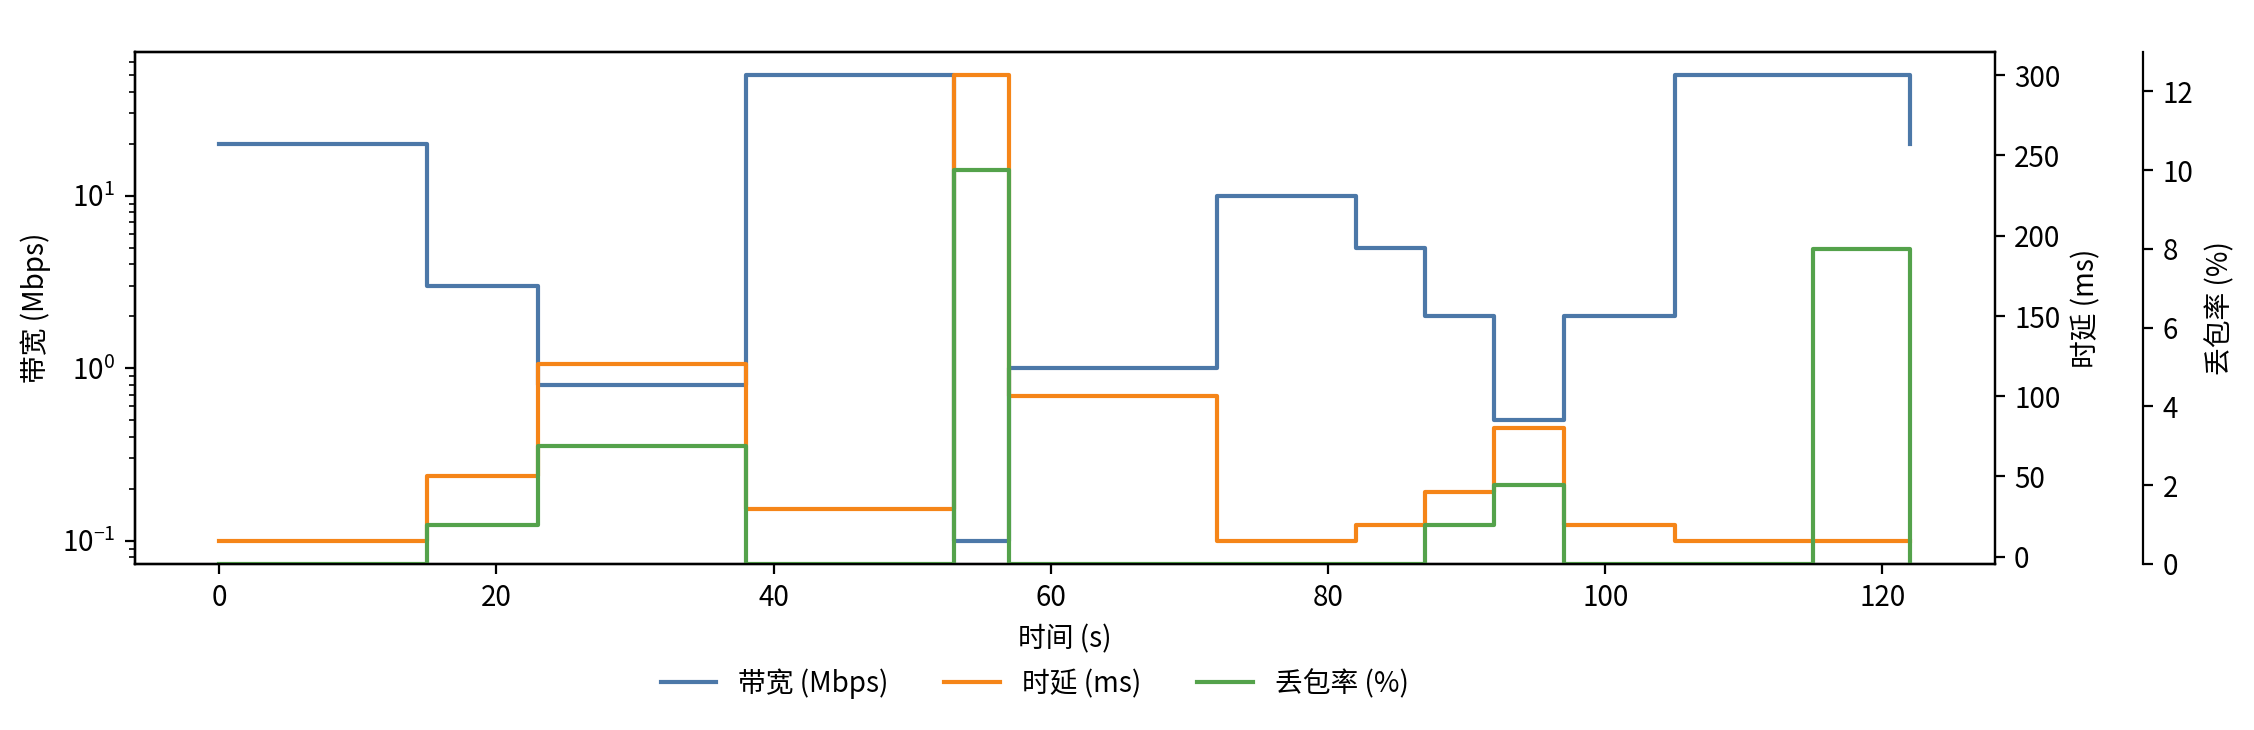
\includegraphics[width=0.95\textwidth]{figures/chapter6/fluctuating_paramters.png}
    \caption{\texttt{fluctuating} 场景：参数时间轴}
    \label{fig:fluctuating-parameters}
\end{figure}

实验链路在两台位于同一局域网的终端设备间建立 WebRTC P2P 连接，每次实验固定使用同一段本地视频以排除内容复杂度的干扰。分组采用随机 50/50 模式，使每次连接在会话开始阶段随机分配到 GCC 或 RL 组，从而降低人为选择偏差。前端通过 \texttt{getStats()} 周期性采集 WebRTC 关键统计量并以 CSV 形式上报落盘。所有场景均采集到对照组与实验组各 10 条 trace，每条 trace 由两端各生成一段 client 统计，单条有效持续时间约 5 分钟。整体测试流程见图~\ref{fig:ab-test-procedure}。

\begin{figure}[htbp]
    \centering
    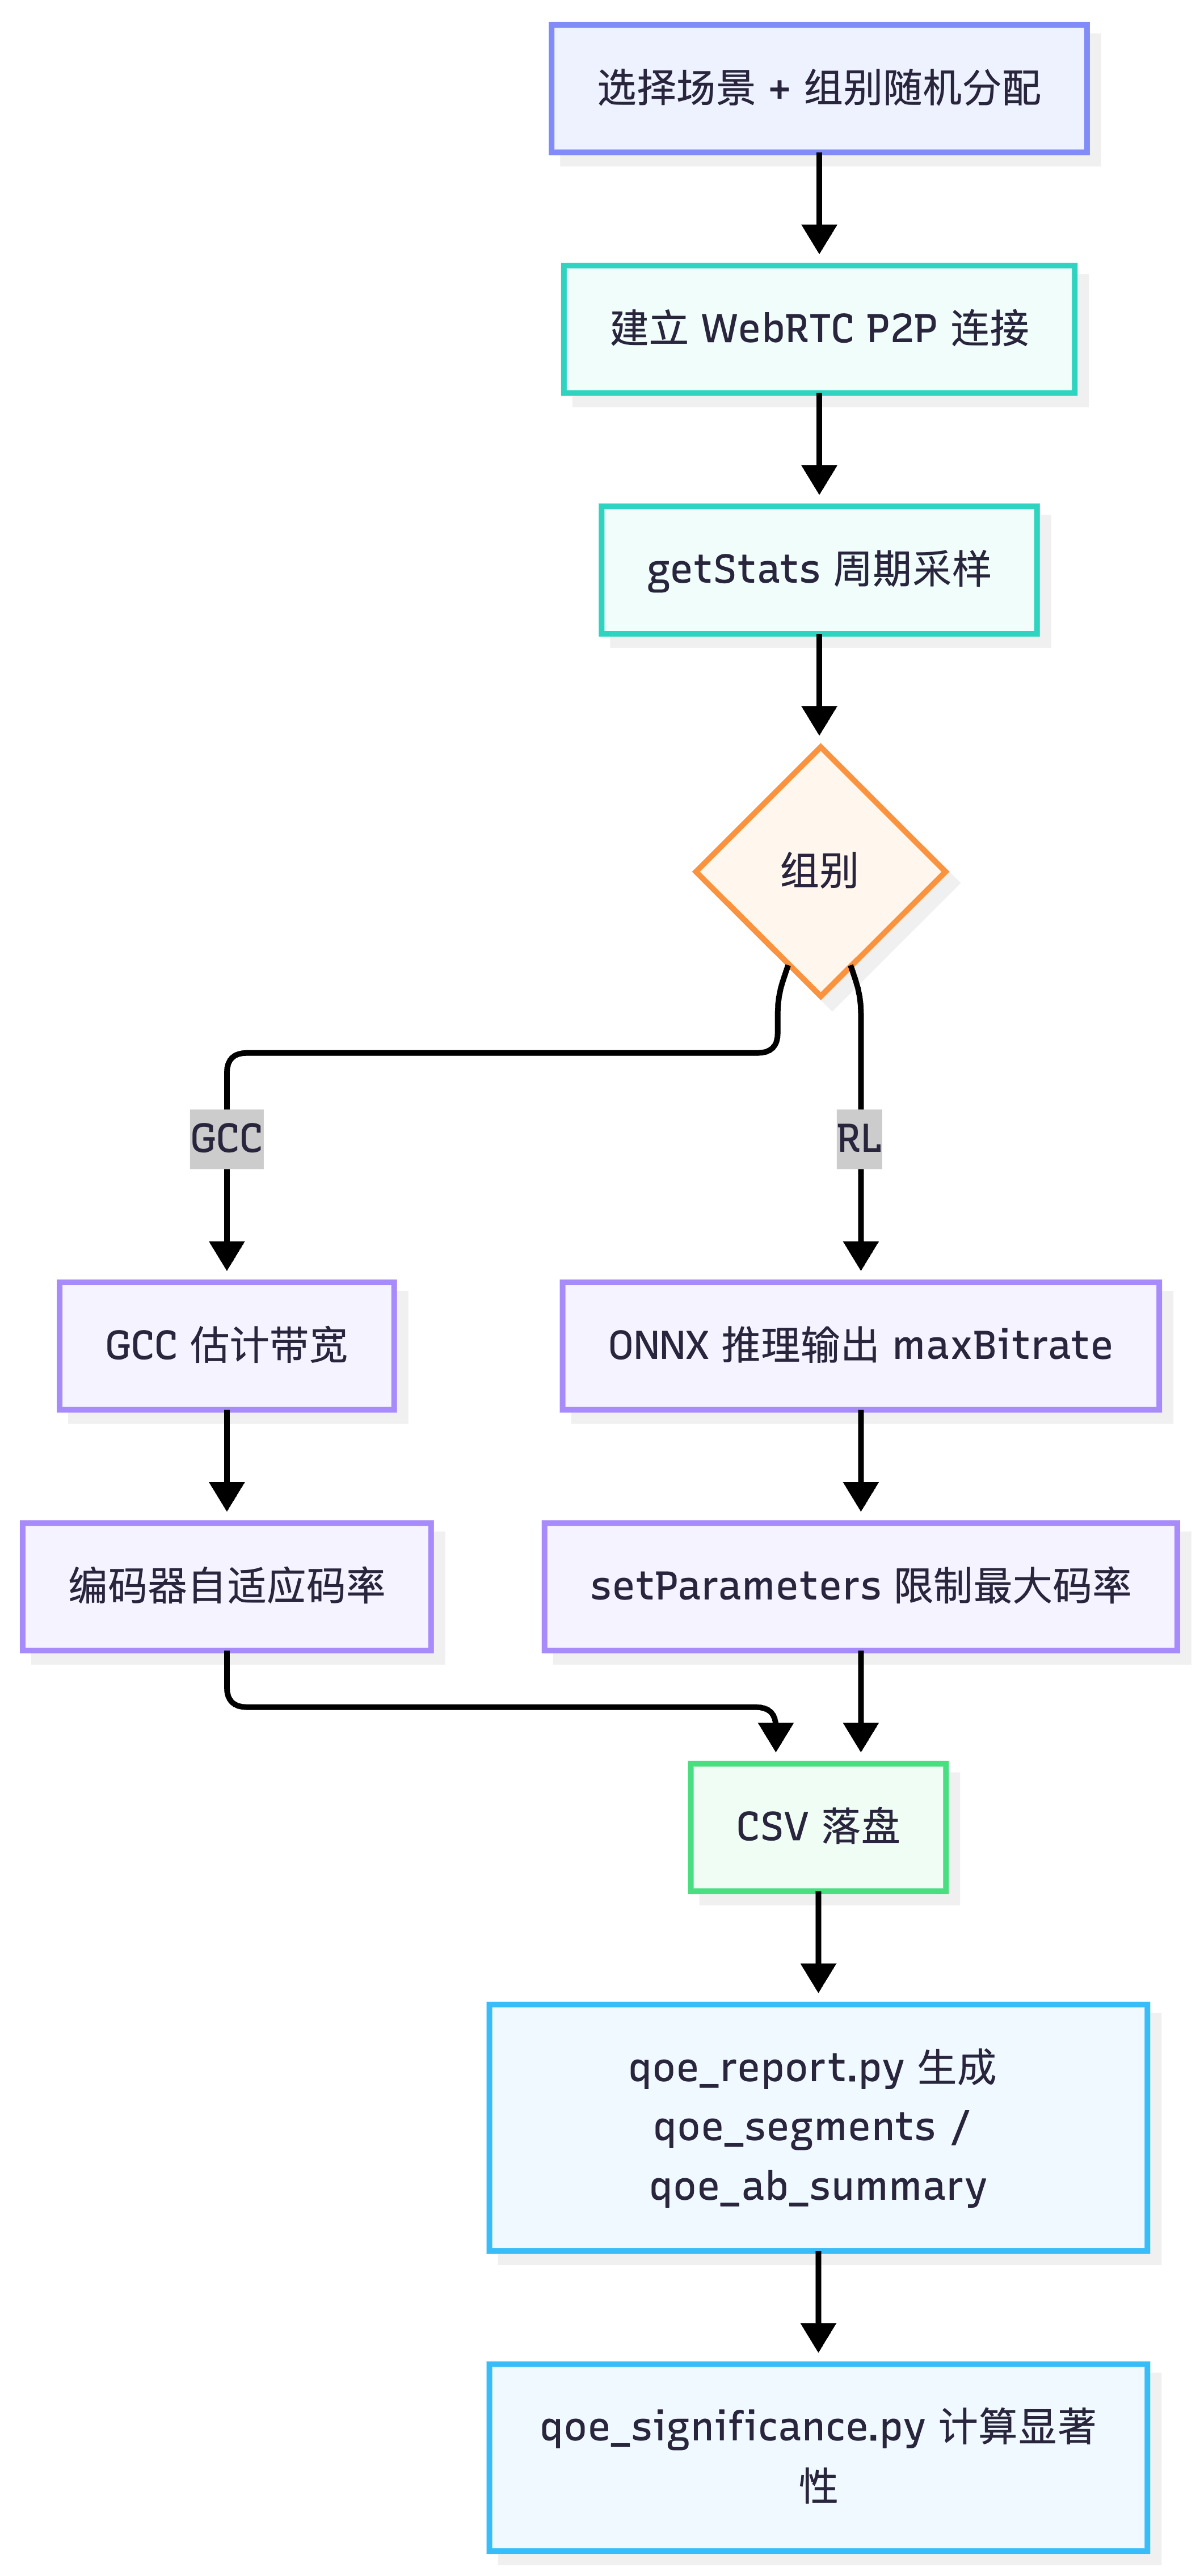
\includegraphics[width=0.6\textwidth]{figures/chapter6/ab_test_procedure.png}
    \caption{A/B 测试流程图}
    \label{fig:ab-test-procedure}
\end{figure}

\section{QoE 评价体系}

为统一量化两种策略在真实链路中的表现，本研究对 A/B 测试采集到的 CSV 轨迹进行两级聚合：先以“单 CSV 文件 + 单 clientId”为单位计算每段会话的 QoE 指标，再按 \texttt{(scenario, ab\_group)} 取均值形成场景级汇总。

评价从五个维度刻画策略性能：吞吐采用接收端 \texttt{recv\_bps} 的均值，时延采用 RTT 的 95 分位以反映尾部交互劣化，抖动采用 \texttt{jitter} 的 95 分位以刻画短时不稳定，丢包采用丢包率均值以反映链路可靠性，动作平滑性则通过有效发送上限 cap 的一阶差分绝对值均值（cap\_delta）刻画码率震荡程度。其中 cap 统一取 \texttt{estimated\_bw\_bps}，其表征的是策略给出的 \texttt{maxBitrate} 与 GCC 估计带宽的最小值，即编码器实际生效的发送上限，从而保证“动作平滑性”评价与真实控制量一致。

综合 QoE 分数采用与第四章奖励函数一致的代理形式：

$$
\mathrm{QoE} = \log\left(1 + \frac{\mathrm{recv\_bps}}{10^6}\right) - \frac{\mathrm{rtt\_ms}}{1000} - \mathrm{loss\_rate} - 0.1 \cdot \frac{|\mathrm{cap}_t - \mathrm{cap}_{t-1}|}{10^6}
$$

该函数以对数项刻画吞吐收益的边际递减，并对时延、丢包与码率震荡施加线性惩罚，从而贴近实时视频通话对“稳定交互”的偏好。

\section{实验结果与分析}

显著性检验以 trace 为单位进行双侧置换检验，文中 p 值均为 BH 校正后的结果。表~\ref{tab:ab-delta-summary} 给出各场景下 RL 相对于 GCC 的关键指标变化（百分比为相对变化率，QoE 以绝对差值表示）。

\begin{table}[htbp]
    \centering
    \small
    \begin{tabular}{|l|c|c|c|c|c|}
        \hline
        场景 & 吞吐变化 & RTT P95 变化 & 丢包率变化 & cap\_delta 变化 & QoE 差值（RL--GCC） \\
        \hline
        baseline & -18.19\% & 0.00\% & 0.00\% & -42.64\% & -0.137 \\
        3g & -3.65\% & -12.42\% & -19.10\% & -73.13\% & +0.054 \\
        dsl & -8.00\% & -7.05\% & -9.02\% & -50.07\% & -0.019 \\
        lte & -3.57\% & -10.82\% & -19.02\% & -73.36\% & +0.189 \\
        low\_bw & -3.17\% & -12.17\% & -19.02\% & -72.77\% & +0.062 \\
        high\_delay & -3.64\% & -11.81\% & -18.97\% & -70.59\% & +0.067 \\
        high\_loss & -3.71\% & -11.68\% & -19.01\% & -70.81\% & +0.018 \\
        fluctuating & -8.27\% & -6.42\% & -9.07\% & -46.06\% & -0.052 \\
        very\_bad & -23.55\% & -16.25\% & -25.14\% & -59.97\% & +0.055 \\
        \hline
    \end{tabular}
    \caption{各场景下 RL 相对于 GCC 的关键指标变化}
    \label{tab:ab-delta-summary}
\end{table}

图~\ref{fig:qoe-score}、\ref{fig:rtt-p95} 与 \ref{fig:loss-rate} 给出各场景下 QoE、RTT P95 与丢包率的分布；图~\ref{fig:cap-delta-cdf} 与图~\ref{fig:throughput-delay-tradeoff} 进一步展示 cap\_delta 全场景 CDF 与吞吐-时延权衡关系。

\begin{figure}[htbp]
    \centering
    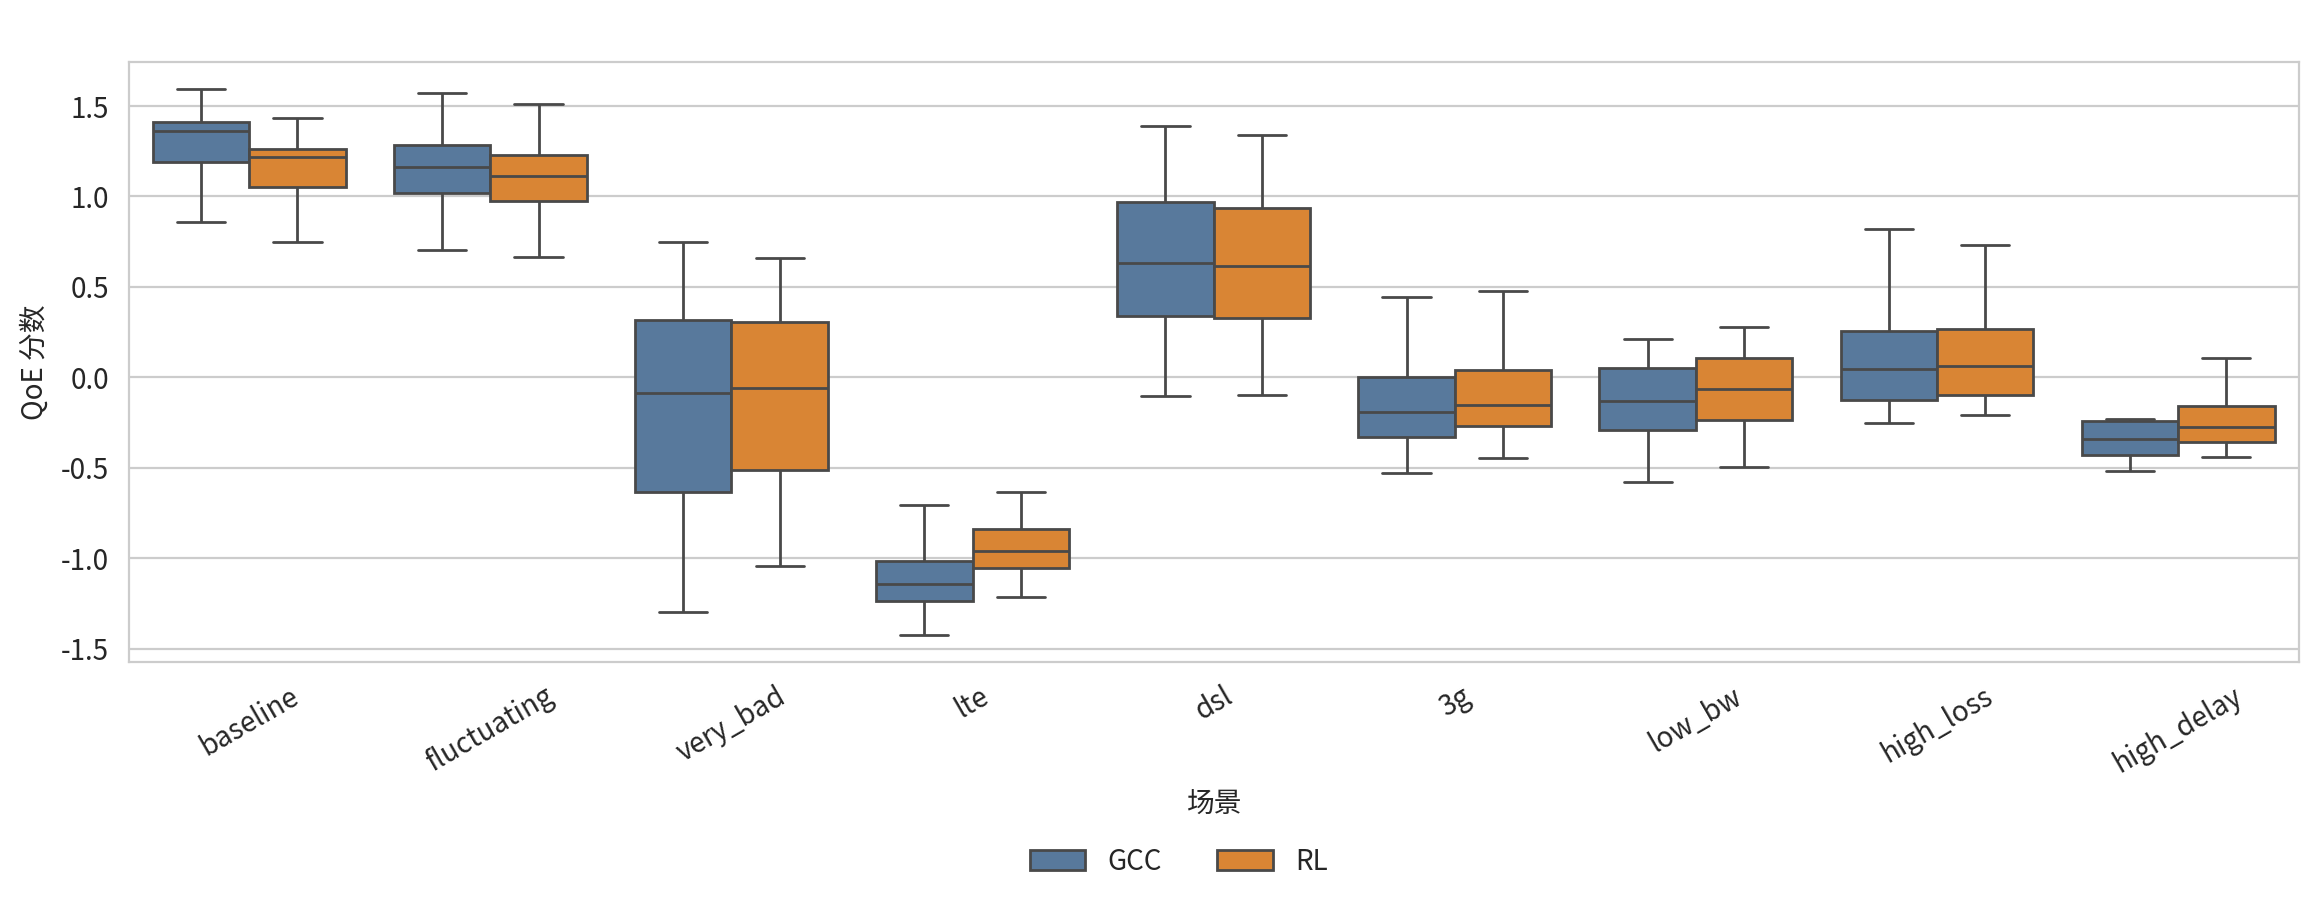
\includegraphics[width=0.9\textwidth]{figures/chapter6/qoe_score.png}
    \caption{QoE 分数分布}
    \label{fig:qoe-score}
\end{figure}

\begin{figure}[htbp]
    \centering
    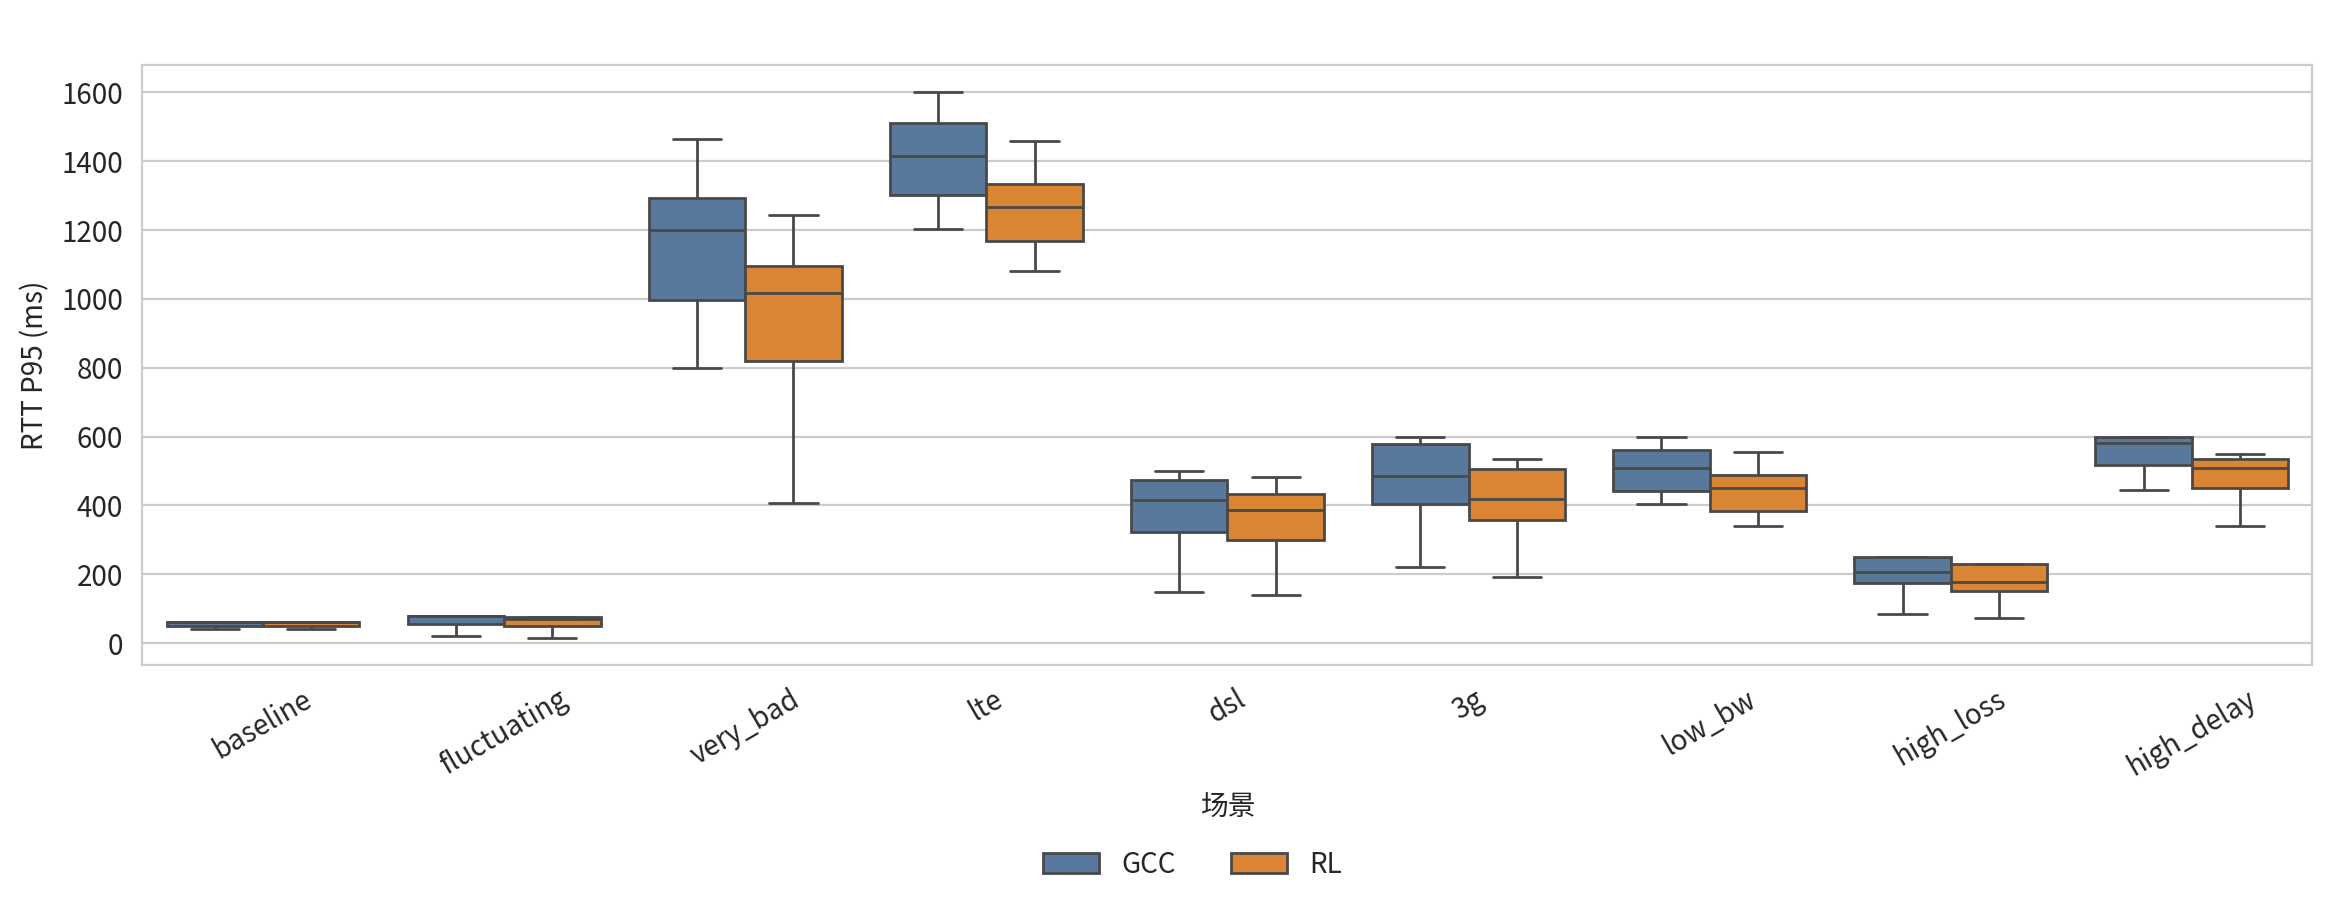
\includegraphics[width=0.9\textwidth]{figures/chapter6/rtt_p95.png}
    \caption{RTT P95 分布}
    \label{fig:rtt-p95}
\end{figure}

\begin{figure}[htbp]
    \centering
    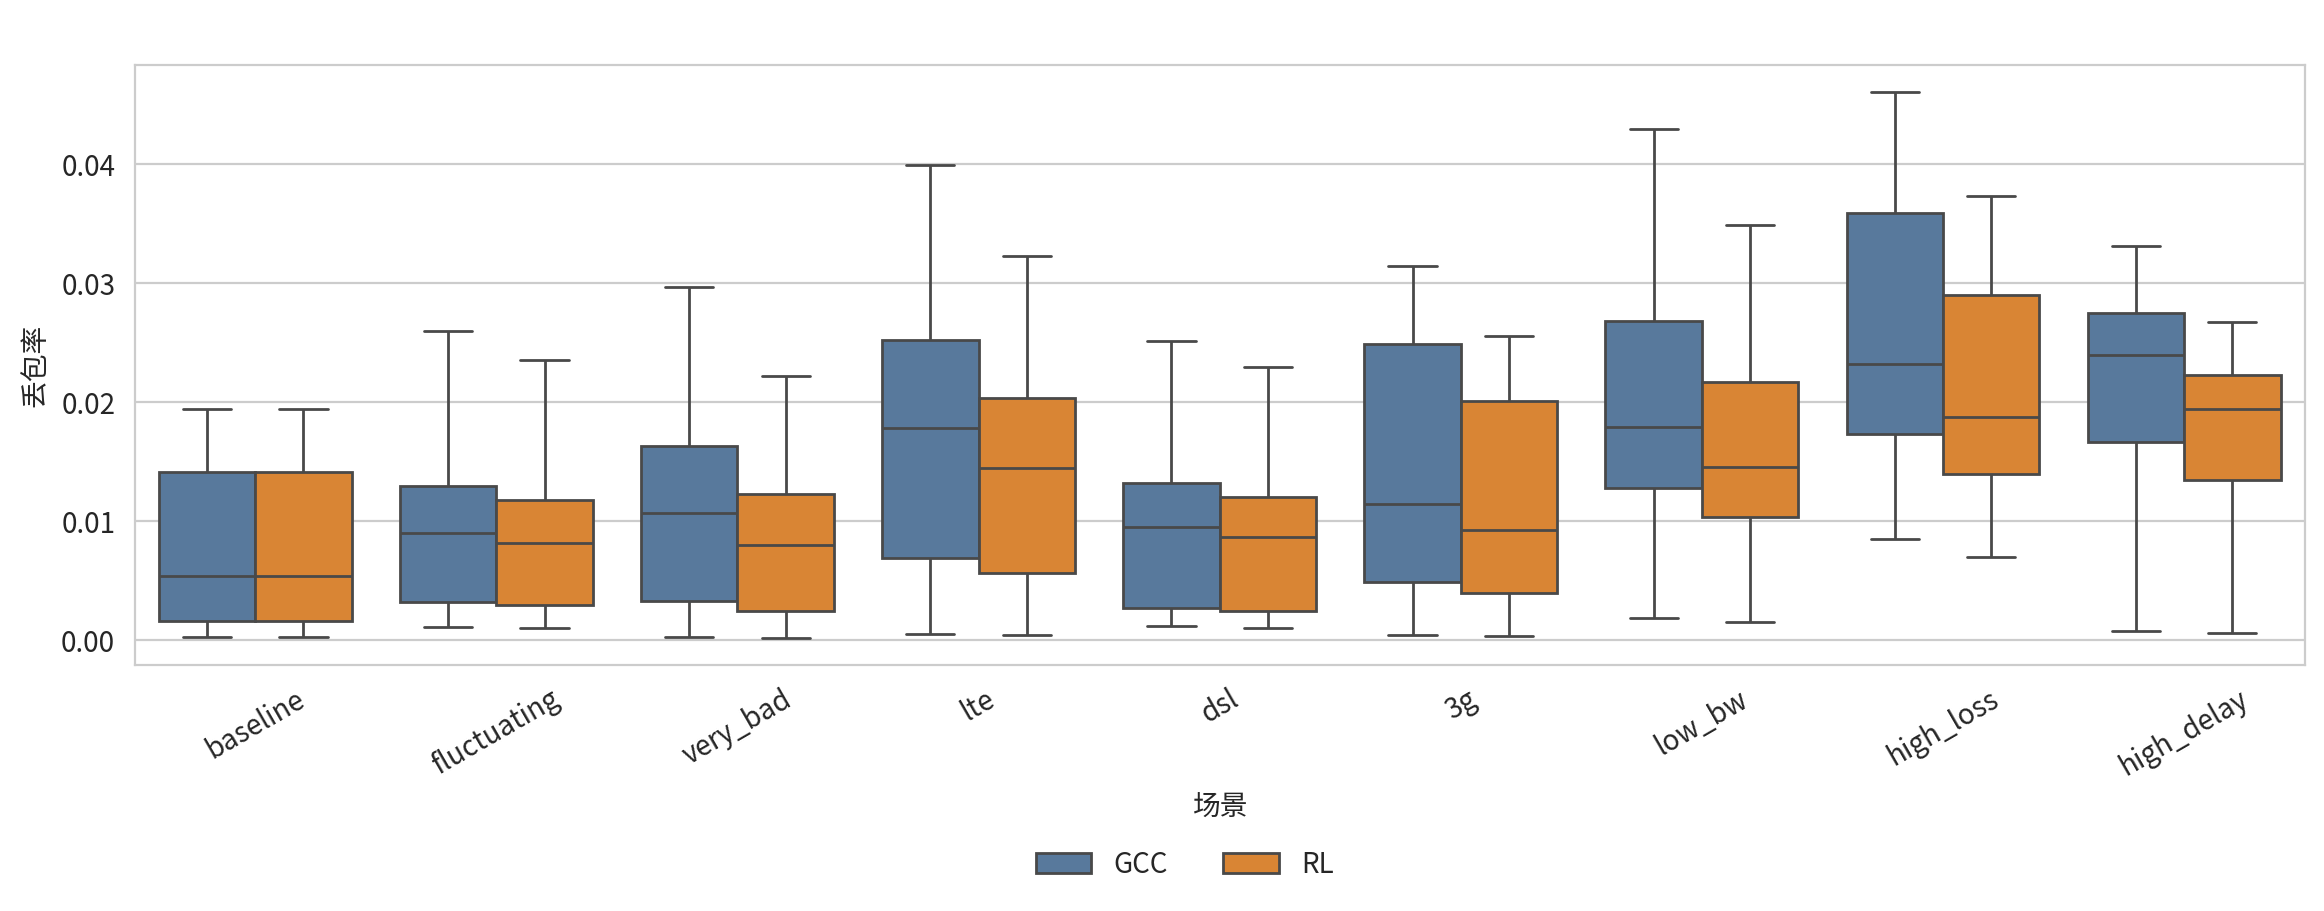
\includegraphics[width=0.9\textwidth]{figures/chapter6/loss_rate.png}
    \caption{丢包率分布}
    \label{fig:loss-rate}
\end{figure}

\begin{figure}[htbp]
    \centering
    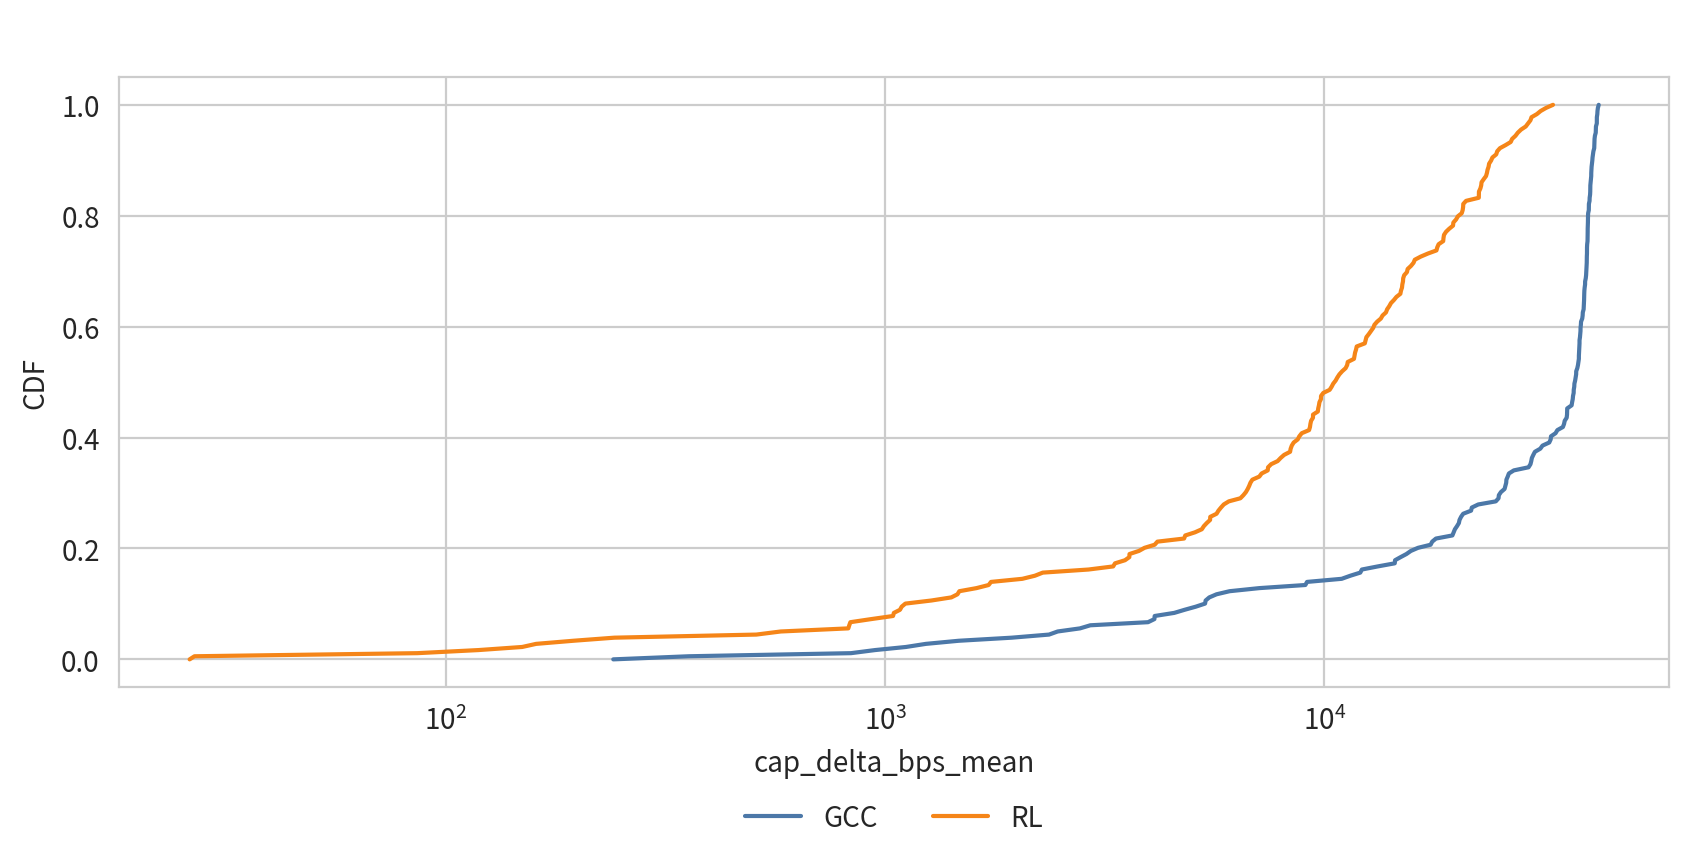
\includegraphics[width=0.9\textwidth]{figures/chapter6/cap.png}
    \caption{cap\_delta 分布 CDF（全场景合并）}
    \label{fig:cap-delta-cdf}
\end{figure}

\begin{figure}[htbp]
    \centering
    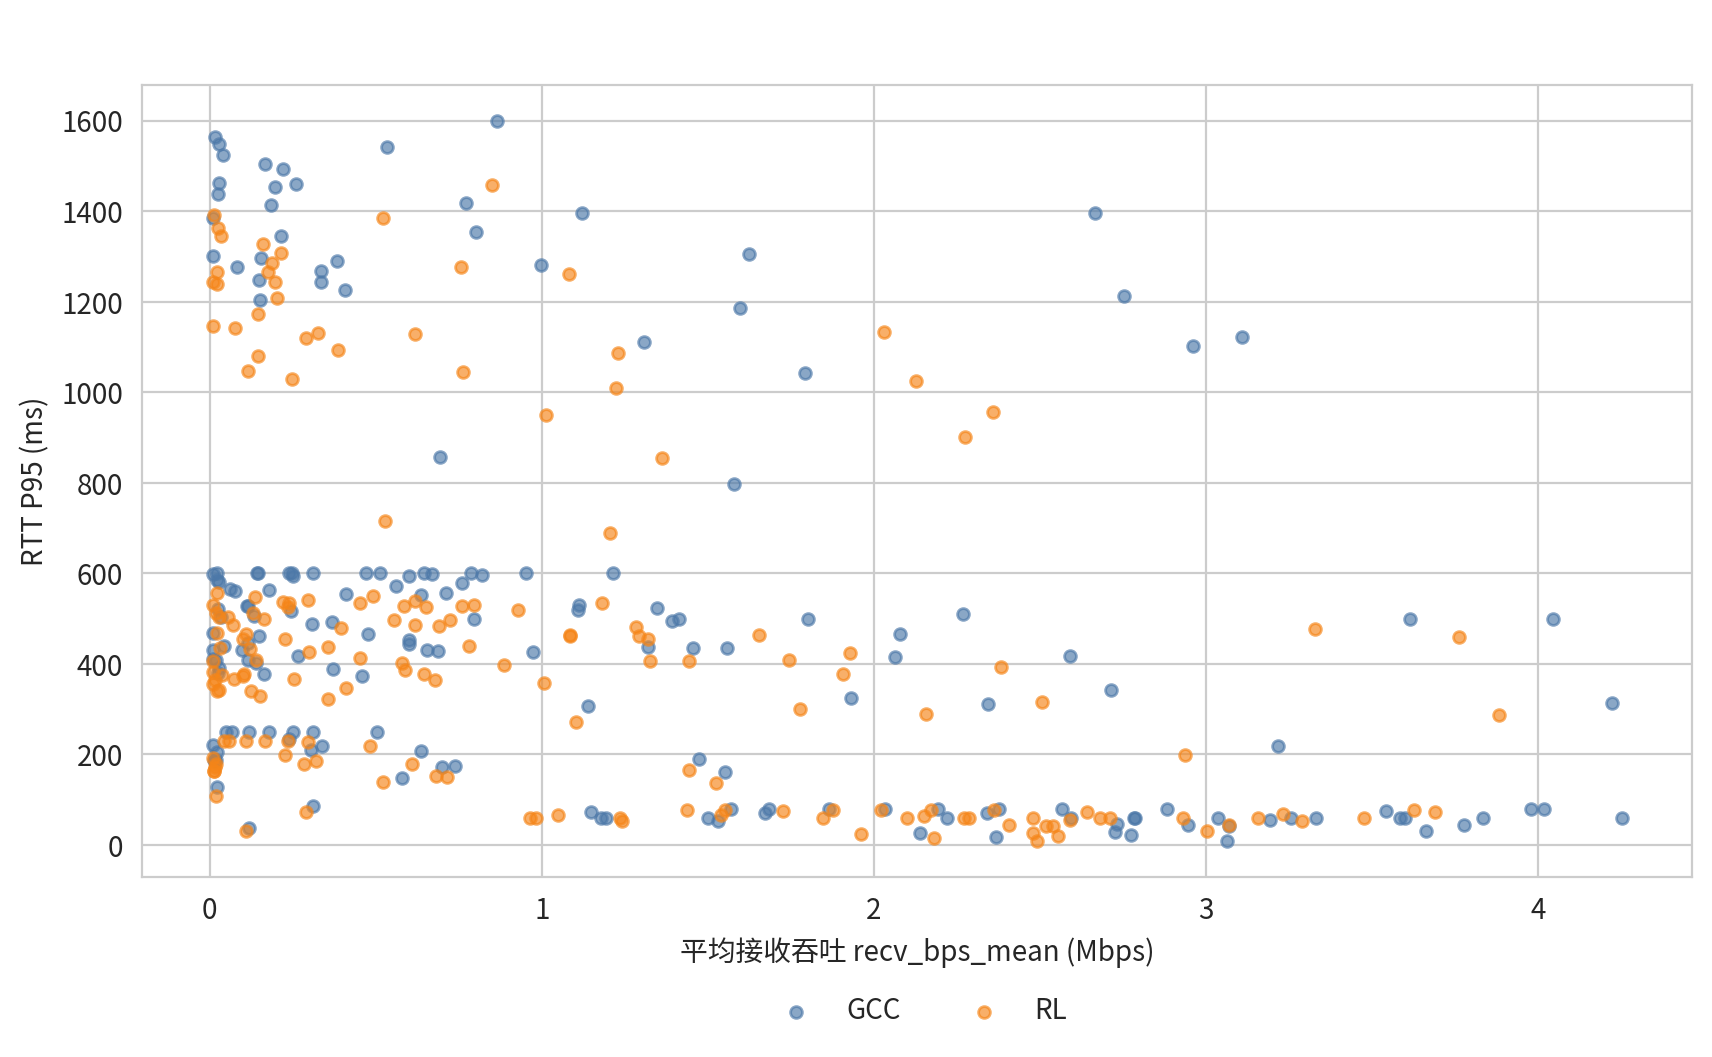
\includegraphics[width=0.9\textwidth]{figures/chapter6/throughtput_delay_tradeoff.png}
    \caption{吞吐-时延权衡散点图}
    \label{fig:throughput-delay-tradeoff}
\end{figure}

整体来看，结果可归纳为三点。其一，动作平滑性在所有场景中均显著下降，下降幅度集中在 42\%--73\%，且 p 值均不超过 0.0012，统计稳健性较强；图~\ref{fig:cap-delta-cdf} 中 RL 组分布整体左移，表明大幅码率跳变出现概率显著降低，能够有效抑制 GCC 在弱网反馈噪声下的“升降—回退”振荡。其二，RTT P95 与丢包率在多数弱网场景中同步降低，3g、lte、low\_bw、high\_delay 与 very\_bad 场景的 RTT P95 下降约 10\%--16\%，丢包率下降约 18\%--25\%，说明策略倾向于通过保守限速避免排队积压；其中 high\_delay、low\_bw 与 lte 场景的 RTT P95 下降已达显著（p 分别为 0.028、0.037、0.026），very\_bad 场景接近显著（p=0.051）。其三，吞吐在多数场景仅有小幅下降，但在 baseline 与 very\_bad 场景出现明显的带宽利用不足；baseline 场景在 RTT 与丢包基本不变的情况下吞吐下降 18\%，QoE 下降 0.137，反映当前策略在高质量网络下存在过度限速倾向。图~\ref{fig:throughput-delay-tradeoff} 印证了该结论：RL 组样本整体向“较低时延、略低吞吐”方向偏移。

进一步聚焦代表性场景。LTE 场景中 RL 将 RTT P95 由 1410 ms 降至 1258 ms，cap\_delta 降低 73\%，综合 QoE 提升 +0.189（p=0.051），可视为收益最明显的“中等带宽 + 较高时延”场景。high\_delay 与 low\_bw 场景中 RL 在吞吐仅下降约 3\% 的前提下显著改善 RTT、丢包与动作平滑性，体现策略以交互稳定性为优先目标的控制偏好。fluctuating 场景中 RL 虽仍降低 RTT 与动作波动，但吞吐下降 8\% 且 QoE 略低于 GCC，其原因在于离线训练数据主要来源于 GCC 行为轨迹，策略对“快速恢复阶段的激进探测”学习不足，加之部署侧引入的 EMA 平滑与单步限幅进一步降低了带宽骤增时的响应速度。

\section{适用性与局限性}

综合上述结果，本文方案的优势体现在三方面。首先，离线强化学习直接利用 GCC 历史轨迹训练策略，避免了在线探索对真实通话造成的质量扰动，并通过 ONNX 与浏览器本地推理形成“采集—训练—部署—验证”的可重复工程闭环，部署风险较低。其次，策略在所有场景下均显著降低 cap\_delta，输出更平滑的带宽上限，有助于减少编码器频繁调参带来的画面抖动，并降低振荡对排队时延与丢包的放大效应。再次，在多类弱网场景中策略呈现一致的降时延与降丢包趋势，体现出对排队积压的主动抑制能力，与离线奖励函数的设计目标相吻合。

由此可推得本方案的适用边界。在 \texttt{3g}、\texttt{lte}、\texttt{low\_bw}、\texttt{high\_delay} 与 \texttt{very\_bad} 等存在带宽瓶颈、高时延或随机丢包的弱网环境下，IQL 策略通过保守且平滑的码率调节获得稳定的 RTT 尾部与丢包率收益，因而尤其适合在线会议、云游戏、远程控制等对交互实时性与稳定性要求高于峰值吞吐的业务。反之，在 \texttt{fluctuating} 这类容量能够快速恢复的场景或大文件传输、超高清点播等以最大化带宽利用率为核心目标的业务中，本模型的保守倾向会限制带宽探测能力，需要通过调整奖励权重或补充高带宽样本进行再训练后再行考虑部署。

本方案仍存在若干局限。其一，QoE 评价函数仅由吞吐、RTT、丢包与动作波动构成，尚未直接覆盖帧率、分辨率切换、卡顿时长等主观体验因素，与真实 MOS 的映射关系仍需进一步验证。其二，每个场景仅含 10 条 trace，且终端类型、浏览器版本与视频内容相对固定，部分指标的统计显著性不足，更大规模与更异构条件下的泛化能力仍待补充验证。其三，baseline 场景的实验结果表明当前奖励权重下策略存在过度保守的倾向，后续可通过引入带宽利用率约束、场景自适应调权或在训练阶段补充高带宽样本加以缓解。其四，离线强化学习本质上仍从行为策略数据中外推决策边界，当真实网络出现训练数据未覆盖的组合模式时，策略可能产生不可预期动作，因此部署侧仍需保留 OOD 检测、动作限幅与回退机制以保障安全性。

\section{本章小结}

本章基于真实 WebRTC 端到端平台构建了覆盖九类典型网络条件的 A/B 测试流程，并以可复现的 QoE 指标体系系统比较了 GCC 与离线强化学习策略。实验结果表明，IQL 策略在多数弱网场景中显著降低码率动作波动并稳定改善 RTT 尾部与丢包率，从而在 LTE、低带宽与高时延等场景获得正向 QoE 收益；与此同时，策略在高质量网络与部分动态恢复场景中存在带宽利用不足，提示后续需在奖励权重、训练数据覆盖与安全约束之间进一步权衡与优化。
